Prova di testo di capitolo. Vorrei citare qui tutta l'opera omnia di~\cite{IEEE:1990,WIKI:INTEROP,BOX:1997,AHL:1996}.

\begin{figure}[tbp] 
\begin{center}
\begin{tabular}{c @{\hspace{1em}} c}
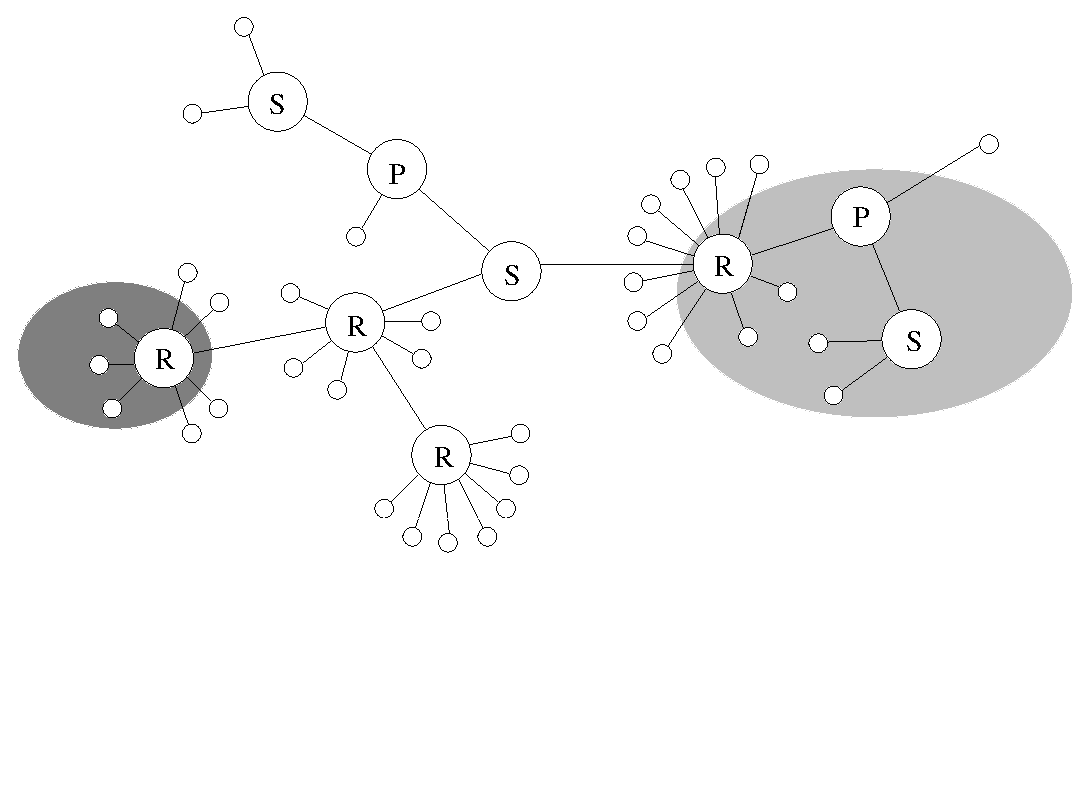
\includegraphics[width=8cm]{figure/esempio-figura-1.eps} &
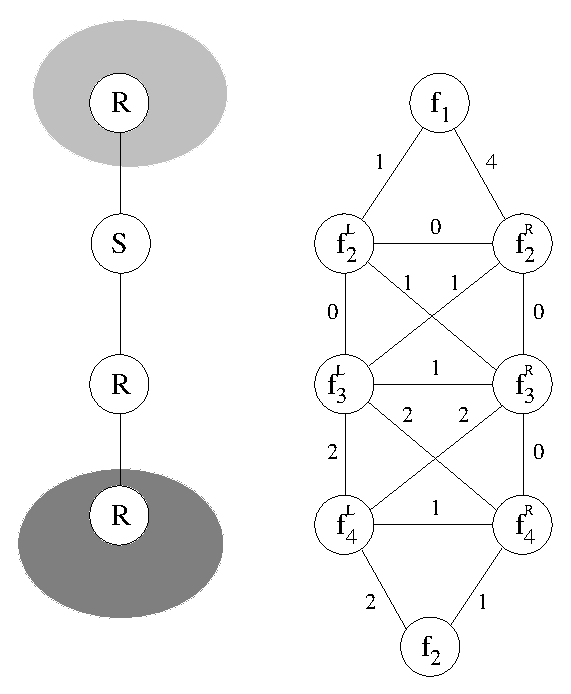
\includegraphics[width=5.5cm]{figure/esempio-figura-2.eps} \\
 (a) & (b)
\end{tabular}
\end{center}
\caption{SPQR-tree di un grafo. (a) L'albero di allocazione della faccia esterna. (b) Il cammino notevole di cui si parla tanto nella Sezione~\ref{se:prima-sezione}.} \label{fig:figura-doppia}
\end{figure}

Come si evince dalle Figure~\ref{fig:figura-doppia}.a e~\ref{fig:figura-doppia}.b non si capisce molto.

\section{La tecnologia Blockchain} % La storia non Nakamoto ma con Napster e il peer2peer 

    \subsection{La vendita del sogno}

    \subsection{Il rovescio della medaglia}

    La macchina infinita di Vitalik (per Etherium) è costruita in che modo?
    %
    Ci interessa sapere come la macchina è costruita perché, in modo molto McLuhanistiano, la macchina forma l'ambiente attorno ad essa. 
    %
    Una \textbf{Blockchain} è composta da due grandi componenti fondamentali: il ledger (libro mastro) e il meccanismo di consenso. 
    %
    Tutte le blockchain attualmente popolari utilizzano un append-only ledger, cioè una nuovo nodo al ledger si aggiunte in coda alla catena e una volta aggiunto è di sola lettura.
    % Questo standard si utilizza solitamente per le attività di log. La blockchain è un'enorme log di transazioni ahahah
    La particolarità è che è decentralizzata, cioè ogni partecipanete elettivo dispone di una completa copia di tutte le transazioni ed è qui che entra in gioco il meccanismo di consenso.
    %
    Tutti i partecipanti validanti, chiamati nodi, hanno una copia completa del database e nessuna delle copie è considerata la copia autorevole.
    %
    Ed è qui che si usa la proof-of-work, in modo da garantire che qualcuno non utilizzi la stessa moneta due volte.


    \section{Cosa resterà dopo lo scoppio della bolla}